\documentclass{standalone}
\usepackage{tikz}
\usetikzlibrary{patterns, positioning}


\begin{document}
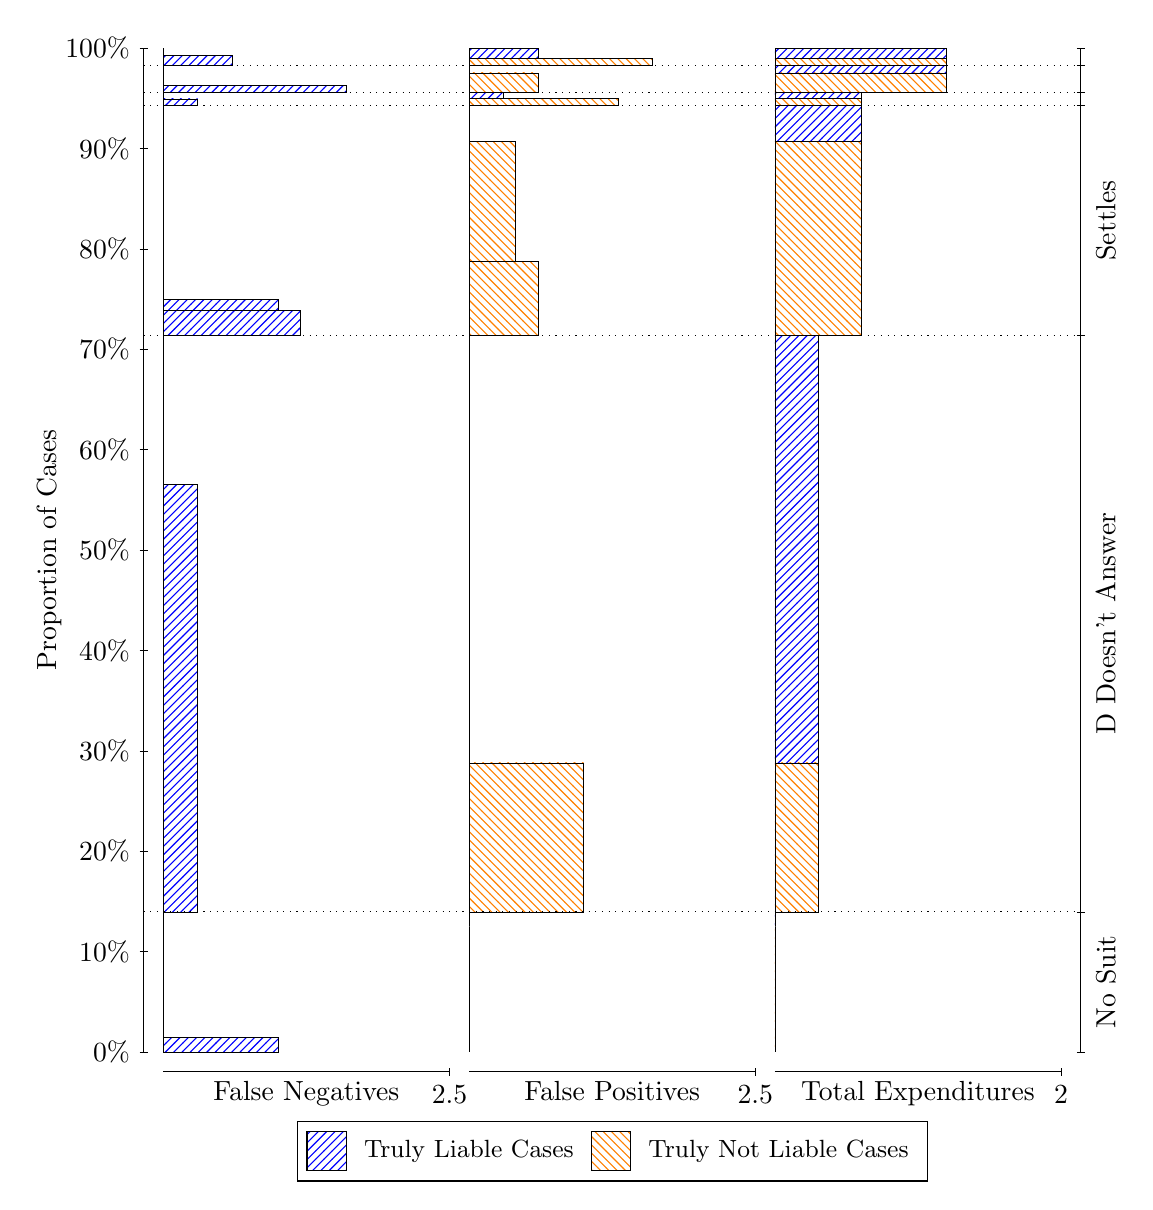
\begin{tikzpicture}
\draw[black, very thin] (1.5,1.75) -- (1.5,14.5);
\node[rotate=90, text=black, anchor=center] at (0.3, 8.125) {Proportion of Cases};
\draw[black, very thin] (1.45,1.75) -- (1.55,1.75);
\node[text=black, anchor=east] at (1.45, 1.75) {0\%};
\draw[black, very thin] (1.45,3.025) -- (1.55,3.025);
\node[text=black, anchor=east] at (1.45, 3.025) {10\%};
\draw[black, very thin] (1.45,4.3) -- (1.55,4.3);
\node[text=black, anchor=east] at (1.45, 4.3) {20\%};
\draw[black, very thin] (1.45,5.575) -- (1.55,5.575);
\node[text=black, anchor=east] at (1.45, 5.575) {30\%};
\draw[black, very thin] (1.45,6.85) -- (1.55,6.85);
\node[text=black, anchor=east] at (1.45, 6.85) {40\%};
\draw[black, very thin] (1.45,8.125) -- (1.55,8.125);
\node[text=black, anchor=east] at (1.45, 8.125) {50\%};
\draw[black, very thin] (1.45,9.4) -- (1.55,9.4);
\node[text=black, anchor=east] at (1.45, 9.4) {60\%};
\draw[black, very thin] (1.45,10.675) -- (1.55,10.675);
\node[text=black, anchor=east] at (1.45, 10.675) {70\%};
\draw[black, very thin] (1.45,11.95) -- (1.55,11.95);
\node[text=black, anchor=east] at (1.45, 11.95) {80\%};
\draw[black, very thin] (1.45,13.225) -- (1.55,13.225);
\node[text=black, anchor=east] at (1.45, 13.225) {90\%};
\draw[black, very thin] (1.45,14.5) -- (1.55,14.5);
\node[text=black, anchor=east] at (1.45, 14.5) {100\%};

\draw[black, very thin] (13.4,1.75) -- (13.4,14.5);
\draw[black, very thin] (13.35,1.75) -- (13.45,1.75);
\node[anchor=west] at (13.35, 1.75) {};
\draw[black, very thin] (13.35,3.5293) -- (13.45,3.5293);
\node[anchor=west] at (13.35, 3.5293) {};
\draw[black, very thin] (13.35,10.848) -- (13.45,10.848);
\node[anchor=west] at (13.35, 10.848) {};
\draw[black, very thin] (13.35,13.775) -- (13.45,13.775);
\node[anchor=west] at (13.35, 13.775) {};
\draw[black, very thin] (13.35,13.938) -- (13.45,13.938);
\node[anchor=west] at (13.35, 13.938) {};
\draw[black, very thin] (13.35,14.275) -- (13.45,14.275);
\node[anchor=west] at (13.35, 14.275) {};
\draw[black, very thin] (13.35,14.5) -- (13.45,14.5);
\node[anchor=west] at (13.35, 14.5) {};

\draw[black, very thin, pattern color=blue, pattern=north east lines] (1.75,1.75) rectangle (3.2033,1.9372);
\draw[black, very thin, pattern color=orange, pattern=north west lines] (1.75,1.9372) rectangle (1.75,3.5293);
\draw[black, very thin, pattern color=blue, pattern=north east lines] (1.75,3.5293) rectangle (2.186,8.955);
\draw[black, very thin, pattern color=orange, pattern=north west lines] (1.75,8.955) rectangle (1.75,10.848);
\draw[black, very thin, pattern color=blue, pattern=north east lines] (1.75,10.848) rectangle (3.494,11.164);
\draw[black, very thin, pattern color=blue, pattern=north east lines] (1.75,11.164) rectangle (3.2033,11.307);
\draw[black, very thin, pattern color=orange, pattern=north west lines] (1.75,11.307) rectangle (1.75,13.775);
\draw[black, very thin, pattern color=blue, pattern=north east lines] (1.75,13.775) rectangle (2.186,13.853);
\draw[black, very thin, pattern color=orange, pattern=north west lines] (1.75,13.853) rectangle (1.75,13.938);
\draw[black, very thin, pattern color=blue, pattern=north east lines] (1.75,13.938) rectangle (4.0753,14.029);
\draw[black, very thin, pattern color=orange, pattern=north west lines] (1.75,14.029) rectangle (1.75,14.275);
\draw[black, very thin, pattern color=blue, pattern=north east lines] (1.75,14.275) rectangle (2.622,14.409);
\draw[black, very thin, pattern color=orange, pattern=north west lines] (1.75,14.409) rectangle (1.75,14.5);
\draw[black, very thin, pattern color=orange, pattern=north west lines] (5.6333,1.75) rectangle (5.6333,3.3421);
\draw[black, very thin, pattern color=blue, pattern=north east lines] (5.6333,3.3421) rectangle (5.6333,3.5293);
\draw[black, very thin, pattern color=orange, pattern=north west lines] (5.6333,3.5293) rectangle (7.0867,5.4221);
\draw[black, very thin, pattern color=blue, pattern=north east lines] (5.6333,5.4221) rectangle (5.6333,10.848);
\draw[black, very thin, pattern color=orange, pattern=north west lines] (5.6333,10.848) rectangle (6.5053,11.794);
\draw[black, very thin, pattern color=orange, pattern=north west lines] (5.6333,11.794) rectangle (6.2147,13.316);
\draw[black, very thin, pattern color=blue, pattern=north east lines] (5.6333,13.316) rectangle (5.6333,13.775);
\draw[black, very thin, pattern color=orange, pattern=north west lines] (5.6333,13.775) rectangle (7.5227,13.86);
\draw[black, very thin, pattern color=blue, pattern=north east lines] (5.6333,13.86) rectangle (6.0693,13.938);
\draw[black, very thin, pattern color=orange, pattern=north west lines] (5.6333,13.938) rectangle (6.5053,14.183);
\draw[black, very thin, pattern color=blue, pattern=north east lines] (5.6333,14.183) rectangle (5.6333,14.275);
\draw[black, very thin, pattern color=orange, pattern=north west lines] (5.6333,14.275) rectangle (7.9587,14.366);
\draw[black, very thin, pattern color=blue, pattern=north east lines] (5.6333,14.366) rectangle (6.5053,14.5);
\draw[black, very thin, pattern color=orange, pattern=north west lines] (9.5167,1.75) rectangle (9.5167,3.3421);
\draw[black, very thin, pattern color=blue, pattern=north east lines] (9.5167,3.3421) rectangle (9.5167,3.5293);
\draw[black, very thin, pattern color=orange, pattern=north west lines] (9.5167,3.5293) rectangle (10.062,5.4221);
\draw[black, very thin, pattern color=blue, pattern=north east lines] (9.5167,5.4221) rectangle (10.062,10.848);
\draw[black, very thin, pattern color=orange, pattern=north west lines] (9.5167,10.848) rectangle (10.607,13.316);
\draw[black, very thin, pattern color=blue, pattern=north east lines] (9.5167,13.316) rectangle (10.607,13.775);
\draw[black, very thin, pattern color=orange, pattern=north west lines] (9.5167,13.775) rectangle (10.607,13.86);
\draw[black, very thin, pattern color=blue, pattern=north east lines] (9.5167,13.86) rectangle (10.607,13.938);
\draw[black, very thin, pattern color=orange, pattern=north west lines] (9.5167,13.938) rectangle (11.697,14.183);
\draw[black, very thin, pattern color=blue, pattern=north east lines] (9.5167,14.183) rectangle (11.697,14.275);
\draw[black, very thin, pattern color=orange, pattern=north west lines] (9.5167,14.275) rectangle (11.697,14.366);
\draw[black, very thin, pattern color=blue, pattern=north east lines] (9.5167,14.366) rectangle (11.697,14.5);
\draw[black, dotted] (1.5,3.5293) -- (13.4,3.5293);
\draw[black, dotted] (1.5,10.848) -- (13.4,10.848);
\draw[black, dotted] (1.5,13.775) -- (13.4,13.775);
\draw[black, dotted] (1.5,13.938) -- (13.4,13.938);
\draw[black, dotted] (1.5,14.275) -- (13.4,14.275);
\draw[black, very thin] (1.75,1.5) -- (5.3833,1.5);
\node[text=black, anchor=north] at (3.5667, 1.5) {False Negatives};
\draw[black, very thin] (5.3833,1.45) -- (5.3833,1.55);
\node[text=black, anchor=north] at (5.3833, 1.45) {2.5};

\draw[black, very thin] (5.6333,1.5) -- (9.2667,1.5);
\node[text=black, anchor=north] at (7.45, 1.5) {False Positives};
\draw[black, very thin] (9.2667,1.45) -- (9.2667,1.55);
\node[text=black, anchor=north] at (9.2667, 1.45) {2.5};

\draw[black, very thin] (9.5167,1.5) -- (13.15,1.5);
\node[text=black, anchor=north] at (11.333, 1.5) {Total Expenditures};
\draw[black, very thin] (13.15,1.45) -- (13.15,1.55);
\node[text=black, anchor=north] at (13.15, 1.45) {2};

\node[text=black, centered, rotate=90] at (13.72, 2.6396) {No Suit};
\node[text=black, centered, rotate=90] at (13.72, 7.1885) {D Doesn't Answer};
\node[text=black, centered, rotate=90] at (13.72, 12.312) {Settles};




\draw (7.449999999999999,1.5) node[draw=none] (baseCoordinate) {};
\begin{scope}[align=center]
        \matrix[scale=0.5, draw=black, below=0.5cm of baseCoordinate, nodes={draw}, column sep=0.1cm]{
            \node[rectangle, draw, minimum width=0.5cm, minimum height=0.5cm, pattern color=blue, pattern=north east lines] {}; &
            \node[draw=none, font=\small, text=black] (B) {Truly Liable Cases}; &
            \node[rectangle, draw, minimum width=0.5cm, minimum height=0.5cm, pattern color=orange, pattern=north west lines] {}; &
            \node[draw=none, font=\small, text=black] (B) {Truly Not Liable Cases}; \\
            };
\end{scope}

\end{tikzpicture}
\end{document}